\documentclass[a4paper]{article}

\usepackage[english]{babel}
\usepackage[utf8]{inputenc}
\usepackage{amsmath}
\usepackage{graphicx}
\usepackage[colorinlistoftodos]{todonotes}
\usepackage{verbatim}

\title{Biogears in Anesthesia Screen Based Simulation}

\author{
  Xiao Han\\
  \and Liewei Ke
  \and Guan Wang
  \and Mclvor William
}

\date{\today}

\begin{document}
\maketitle

\begin{abstract}
The delivery of good medical care concerns patients as well as medical professionals. In terms of medical training, mannequins used to be orthodox way to train and demonstrate medical skills for students. Nowadays, schools and institutions are adopting more and more high-tech involved methodologies such as Simulation-Based medical education, Virtual Reality in order to provide students with immersive and realistic experience of medical training. In Simulation-Based medical education particularly, whether the models of physiology incidents or responses are accurate or not will directly affect the credibility of the simulation. In this paper, we will give insights into the physiology simulation and compare the current physiology engine Biogears. We will evaluation its function by comparing with simulation provided by CAE Muse system. In the end, we will conclude on the performance of Biogears on key points such as authenticity, stability as well as commenting on its limitations.
\end{abstract}

\section{Current physiologic engines and BioGears}
There are a lot of physiologic engines or simulation softwares out there that provides ability to simulate sophisticated body systems. Some of them are licensed so medical schools or institutions will have to buy them for usage. For example, CAE is a simulation company that provides simulation for aviation, security(defense) and healthcare. Their main product for medical simulation is Muse. Must provides several simulation scenarios where patients come with different conditions.

Biogears is an open-source physiology engine that provides accurate as well as consistent physiologic simulation of human bodies. It contains models that mimic human systems as circuits and substance in physiology for real-time input. It can be used as standalone application where physicians could use integrated GUI to simulate customized scenarios or integrated with mannequins, sensors or interfaces that utilize the engine to output consistently.

To thoroughly evaluate Biogears simulation, we repeatedly conducted several experiments on normal patients and calculate key variables within the patients. We evaluate engine stability by calculating the mean squared error of several vital signs. We evaluate engine authenticity by comparing with CAE simulation result and consulting with real doctors and physicians.  



\section{Show equivalence to current training methods}

- how to show current training methods

\subsection{Current training methods}
\subsection{Why using screen based simulation is equivalent to current training methods}

\section{Show physiologically appropriate, responses to key events}

The reason why physicians don't buy into simulation-based software is due to the fundamental distrust in the models simulation software utilized to generate all the signals and data. And yet, there is no uniformly consented algorithms to describe the complicated nature of human bodies. Thus, the most reliable way to evaluate whether a simulation is fit for real scenario operations is to compare them with the common sense of physicians and doctors. For example, one of the most common thoughts of physicians about the authenticity of scenarios generated by simulation is to see the heart rate of patient when the patient is given different dosage of morphine. If you inject a small dosage of morphine it should somehow make the patient calm down and reduce the heart rate but if you inject more morphine than you should, the drug may be likely to kill a patient. 

Inspired by the previous work from this paper \cite{measure_repeatability}, we think the quality of a simulation system will also be determined by the stability of experiments under the same or similar circumstances. After consulting with physicians from UPMC and Biogears team, we enumerate several representative experiments and ran both Biogears and CAE simulation on them. Later we presented the result in graphs and tables for visuality.

\subsection{Bleeding Out Scenarios}

Bleeding patients are often seen in trauma and emergency rooms. The cause of this symptom varies. Car accident, Blood vessel abnormalities, blood disorders, tumors, to name a few. We believe that to see how simulation engine reacts to a patient who is suffering from bleeding would be a good way to see how it models human bodies change as time goes by.

To run this experiment on Biogears, we tested it using built-in GUI of Biogears that provides dozens of substances simulation.  

\begin{figure}[!htb]\centering
   \begin{minipage}{0.49\textwidth}
     \frame{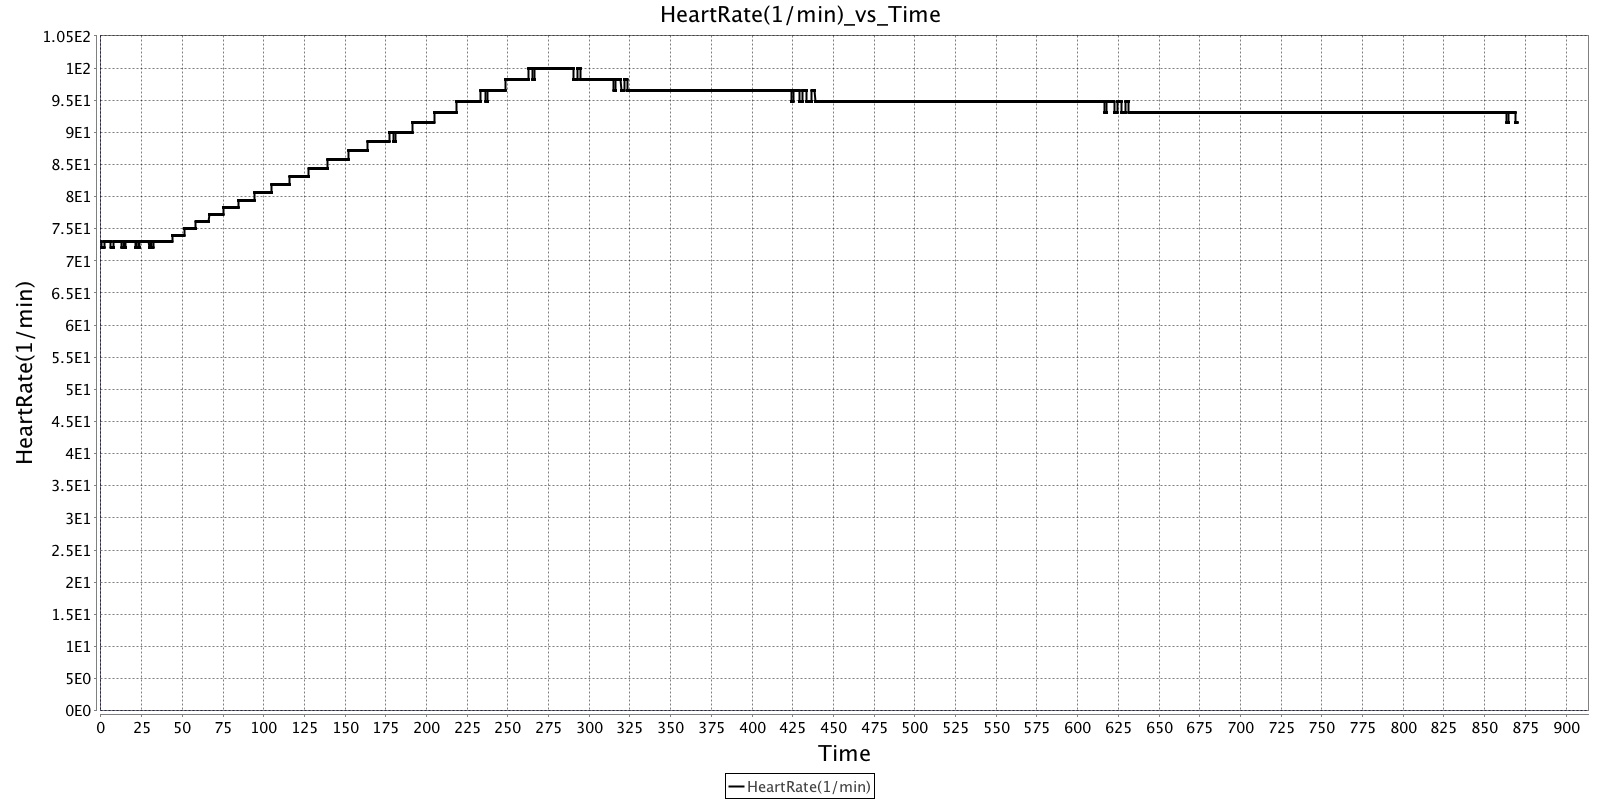
\includegraphics[width=5cm]{bleeding_out_HeartRate_vs_Time.jpg}}
     \caption{heart rate changes}
     \label{fig:patient bleeding}
     
   \end{minipage}
   \begin {minipage}{0.49\textwidth}
     \frame{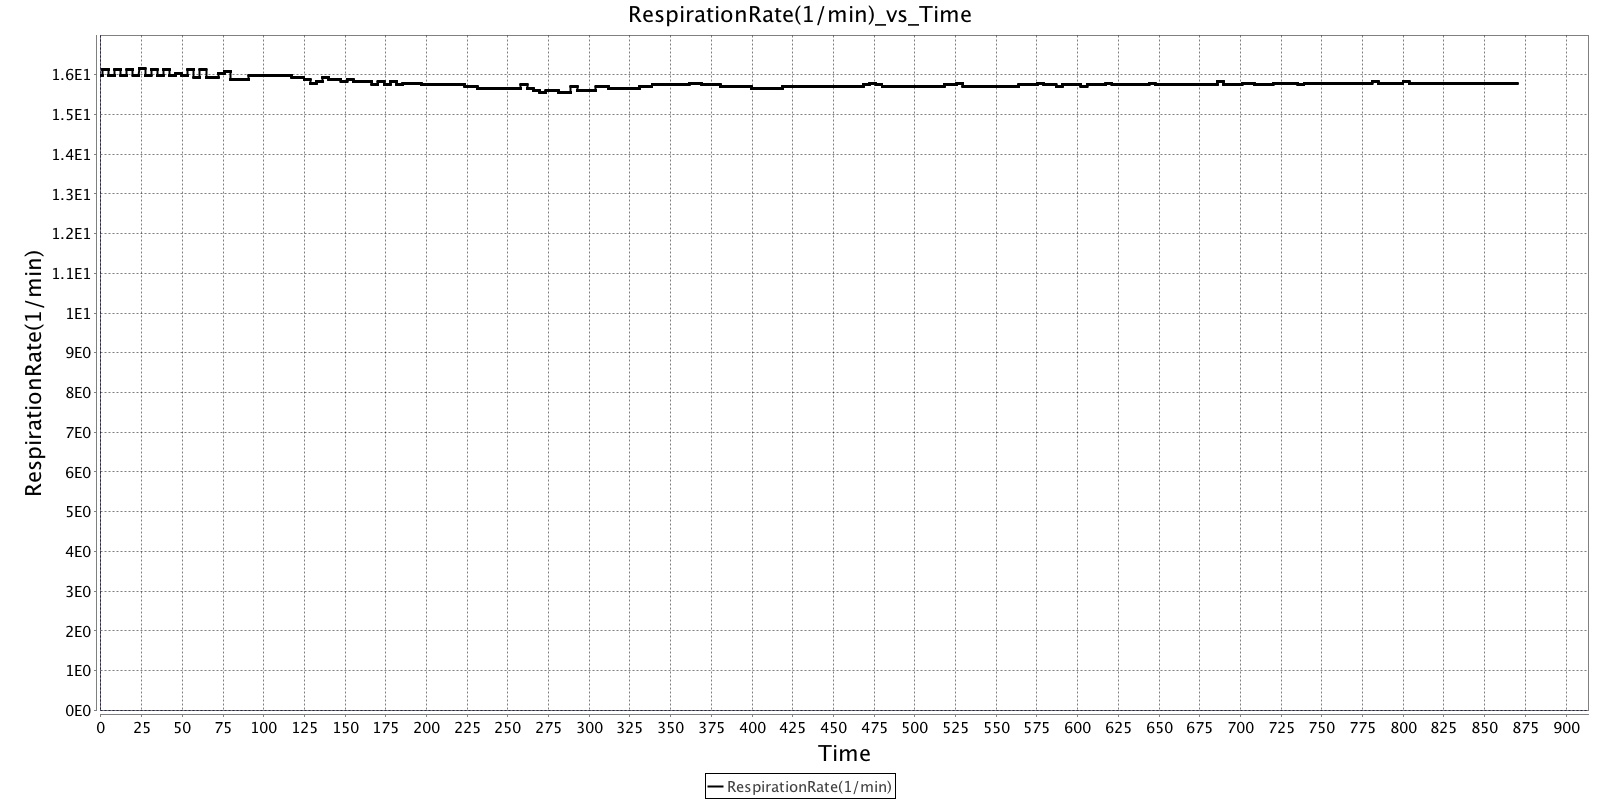
\includegraphics[width=5cm]{bleeding_out_RespirationRate_vs_Time.jpg}}
     \caption{respiratory rate changes}
     \label{fig:patient bleeding}
   \end{minipage}
\end{figure}

In reality, it is not the case that patient could live with continuous hemorrhage: The heart rate of patient will increase because with blood loss there is not enough oxygen so his/her heart has to pump faster and absorb more oxygen. His respiratory rate will rise. But after a while, when he/she eventually loses


- bleeding out scenarios, multiple experiments, (mean, root mean squared error, median performance error data recorded)
- oxygen desaturation (same as aboved)

- patient stop breathing for 30 seconds, 2 mins and recover

- (optional) compare with another dataset asac dataset

- simulate with propofal(200mg), morphine so4(20mg), rocuromium(50mg), succinocloon(100mg), room air(170/70kg)

\subsection{Oxygen Desaturation Scenarios}

Oxygen Desaturation is another incident that's often observed by physicians where it occurs during sleep of patients with chronic obstructive lung disease and is often caused by sleep-disordered breathing(SDB)\cite{low_oxygen_sleep}. When this happens, the concentration of oxygen in patients' blood decreases and it may result in various symptoms, such as shortness of breath.

For physicians, being able to track how long patient has been experiencing such symptoms is important. For example, in surgery, if patient suffered from deficiency of blood oxygen for a long time, it may cause their brains irreversible damage. So we also designed experiments to see how Biogears reacts to patients simulation who are suffering from lack of oxygen for different range of time. In reality, if a patient experience lack of oxygen in blood for a longer time, it will be harder or even impossible for his brain and body to recover from this disease.

In Biogears, we set up two patients to stop breathing for 30 and 120 seconds and then restore the their air supply. The following graphs are the simulation result for them.

\begin{figure}[!htb]\centering
   \begin{minipage}{0.49\textwidth}
     \frame{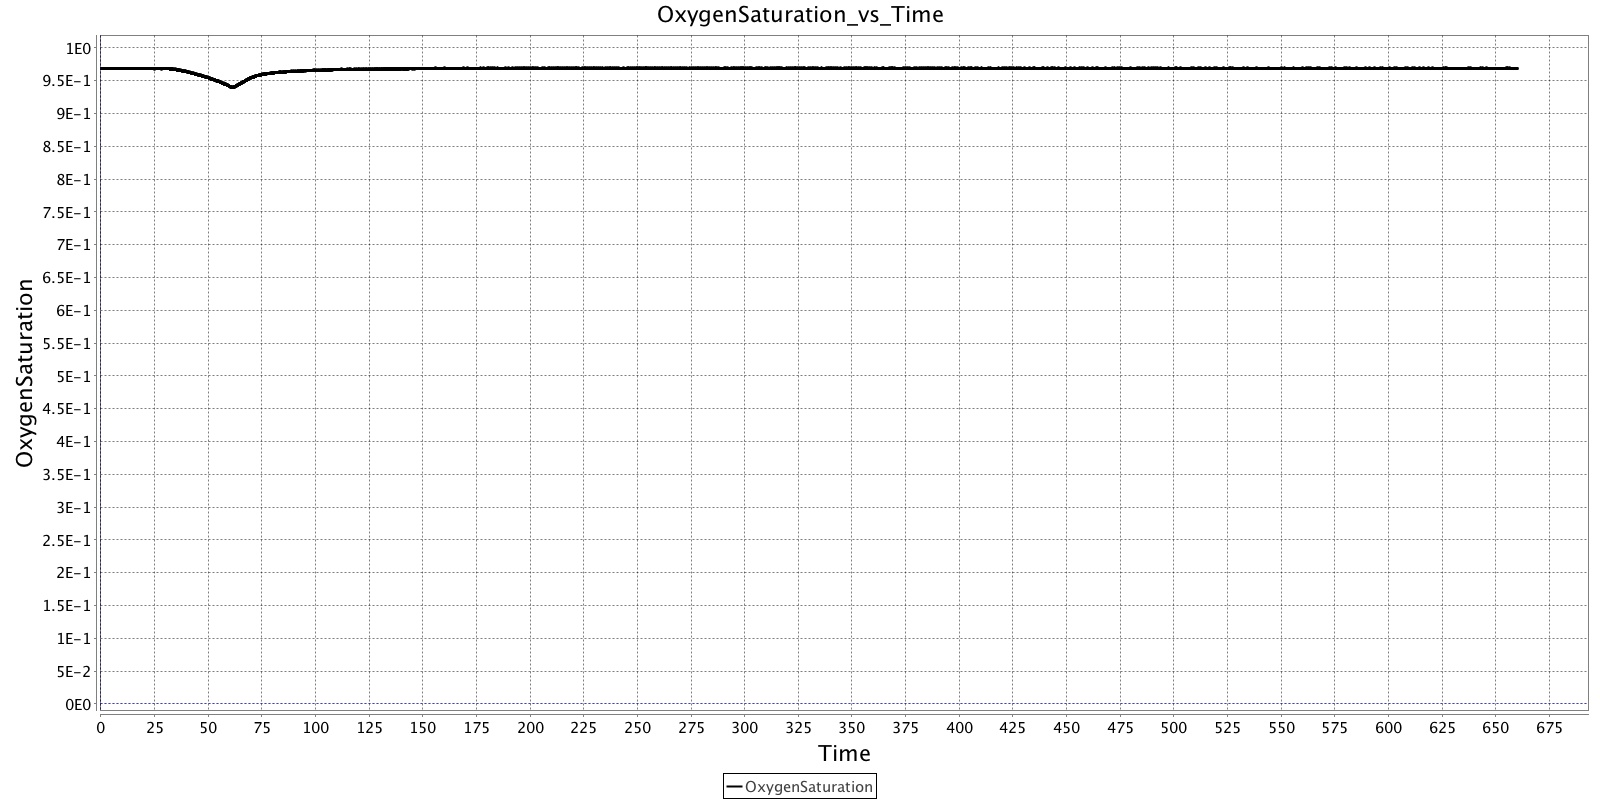
\includegraphics[width=5cm]{30_OxygenSaturation_vs_Time.jpg}}
     \caption{oxygen saturation changes}
     \label{fig:patient stoping breathing}
     
   \end{minipage}
   \begin {minipage}{0.49\textwidth}
     \frame{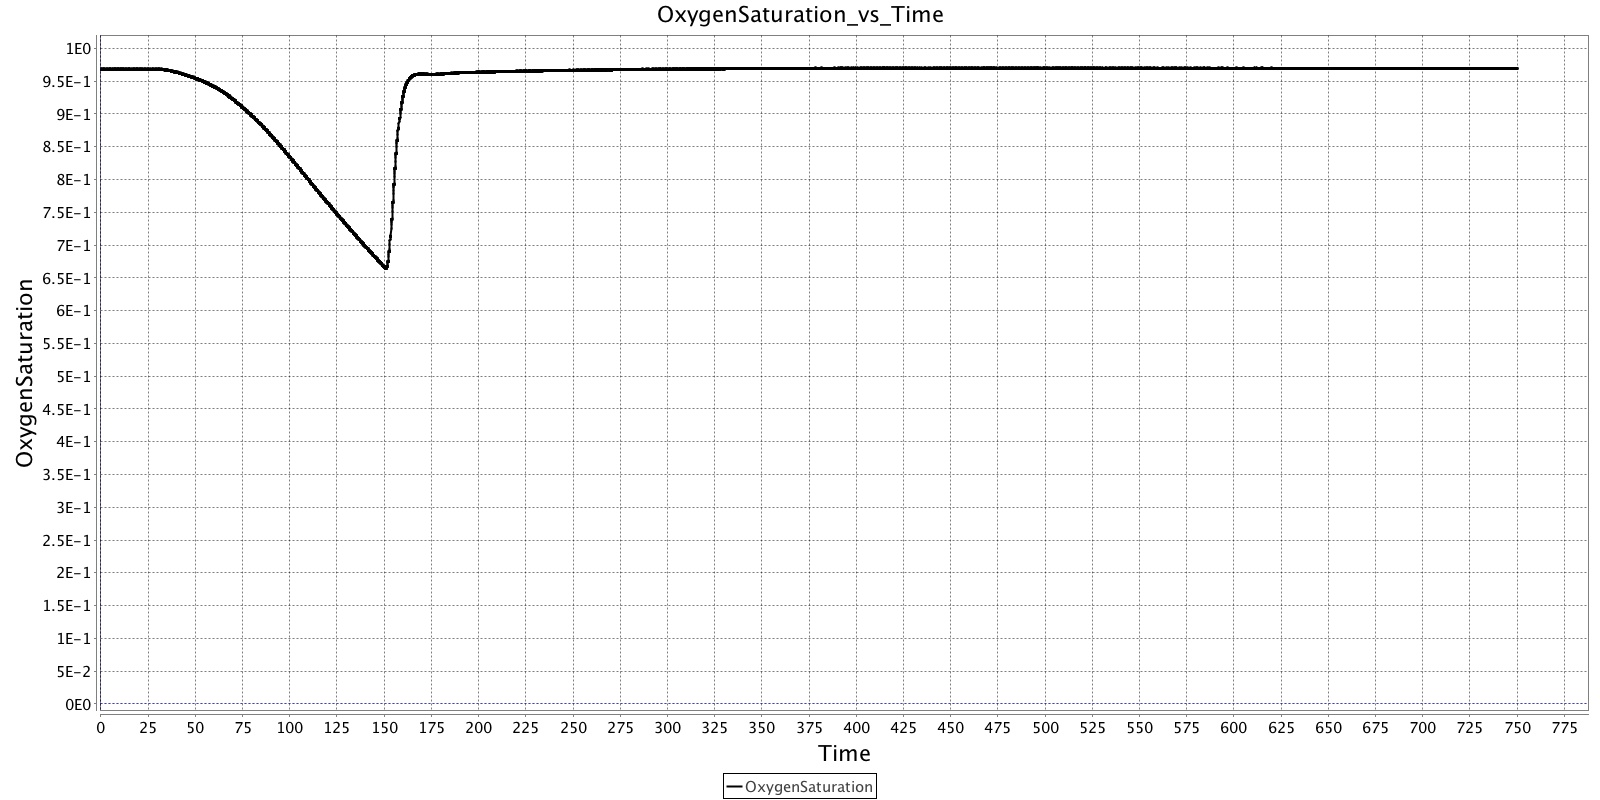
\includegraphics[width=5cm]{120_OxygenSaturation_vs_Time.jpg}}
     \caption{oxygen saturation changes}
     \label{fig:patient stoping breathing}
   \end{minipage}
\end{figure}

As we can see on the graphs, both patients' oxygen saturation drops as they stopped breathing and once we restore the air supply, they recovered from it in 25 seconds. And there actually isn't difference in how long it will take them to recover from the deficiency. It shows that Biogears is currently not capable of simulating this complex yet delicate recovery scenarios.

\subsection{Tests for Common Drugs}

\subsubsection{Succinycholine Simulation}

Succinycholine is a drug that could trigger short-period muscle relaxation and therefore used as an approach to induce short-period paralysis. In the discipline of anesthesia, it is used widely for emergency medicine and trauma care due to its fast-acting and short-duration nature. Therefore, adjusting its dosage to multiple scenarios is important for those who wish to practice their knowledge and become anaesthetist in the future.

In Biogears, we set up the Succinycholine's dosage to be 5 mg as suggested by Dr. Mchvor. We simulated the scenario for  
more than 900 seconds cause it takes time for patient to recover from paralysis.

When observing the result graphs, we could see that patient stopped breathing for nearly 4 minutes. 

\begin{figure}[!htb]\centering
   \begin{minipage}{0.49\textwidth}
     \frame{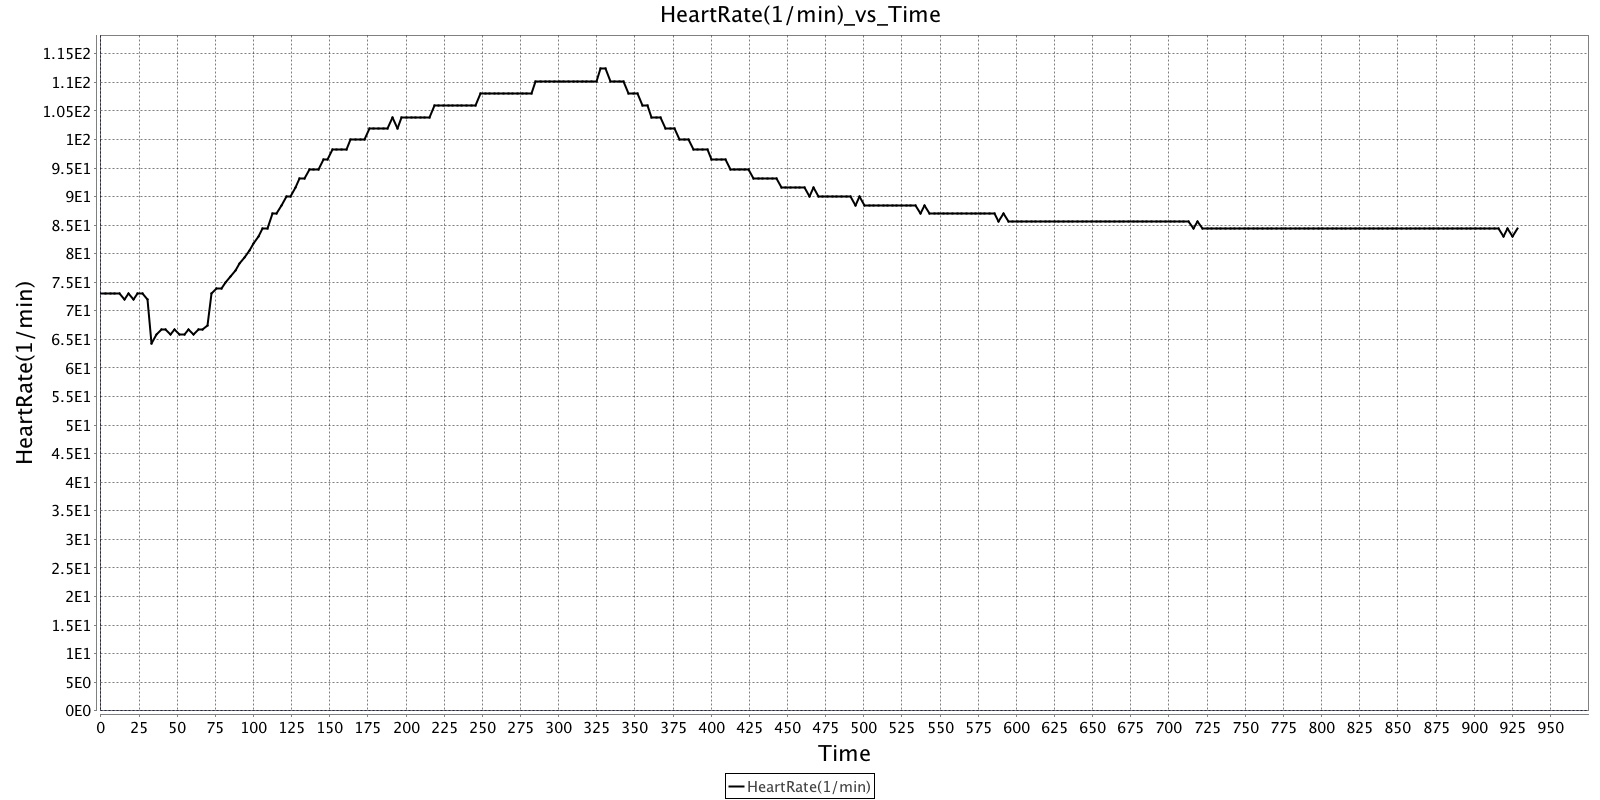
\includegraphics[width=5cm]{Succinylcholine_HeartRate_vs_Time.jpg}}
     \caption{Heart Rate changes}
     \label{fig:given 5 mg Succinylcholine}
     
   \end{minipage}
   \begin {minipage}{0.49\textwidth}
     \frame{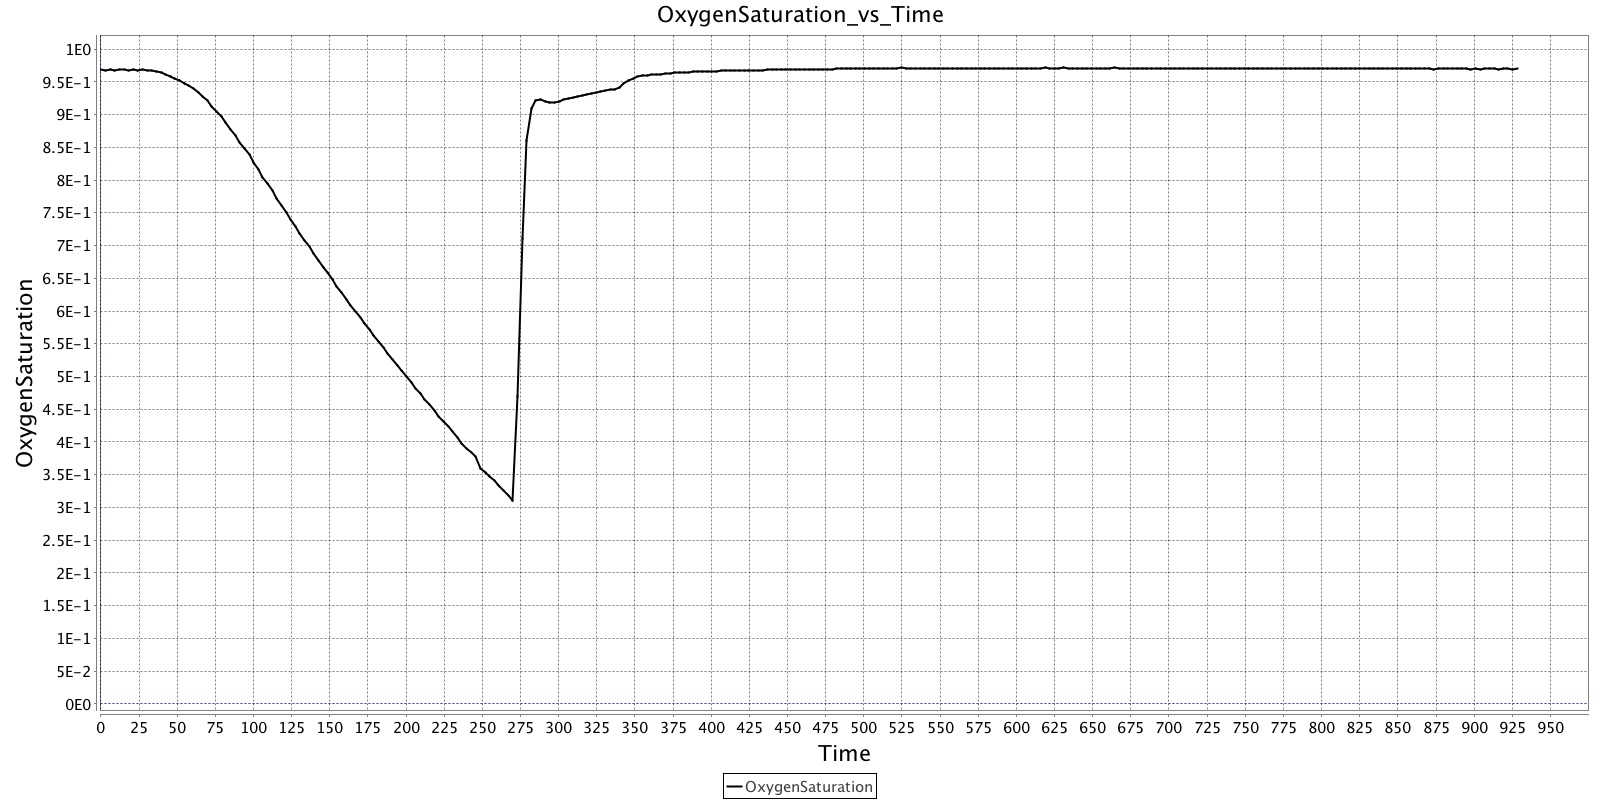
\includegraphics[width=5cm]{Succinylcholine_OxygenSaturation_vs_Time.jpg}}
     \caption{Oxygen Saturation changes}
     \label{fig:given 5 mg Succinylcholine}
   \end{minipage}
\end{figure}

\begin{figure}[!htb]\centering
   \begin{minipage}{0.49\textwidth}
     \frame{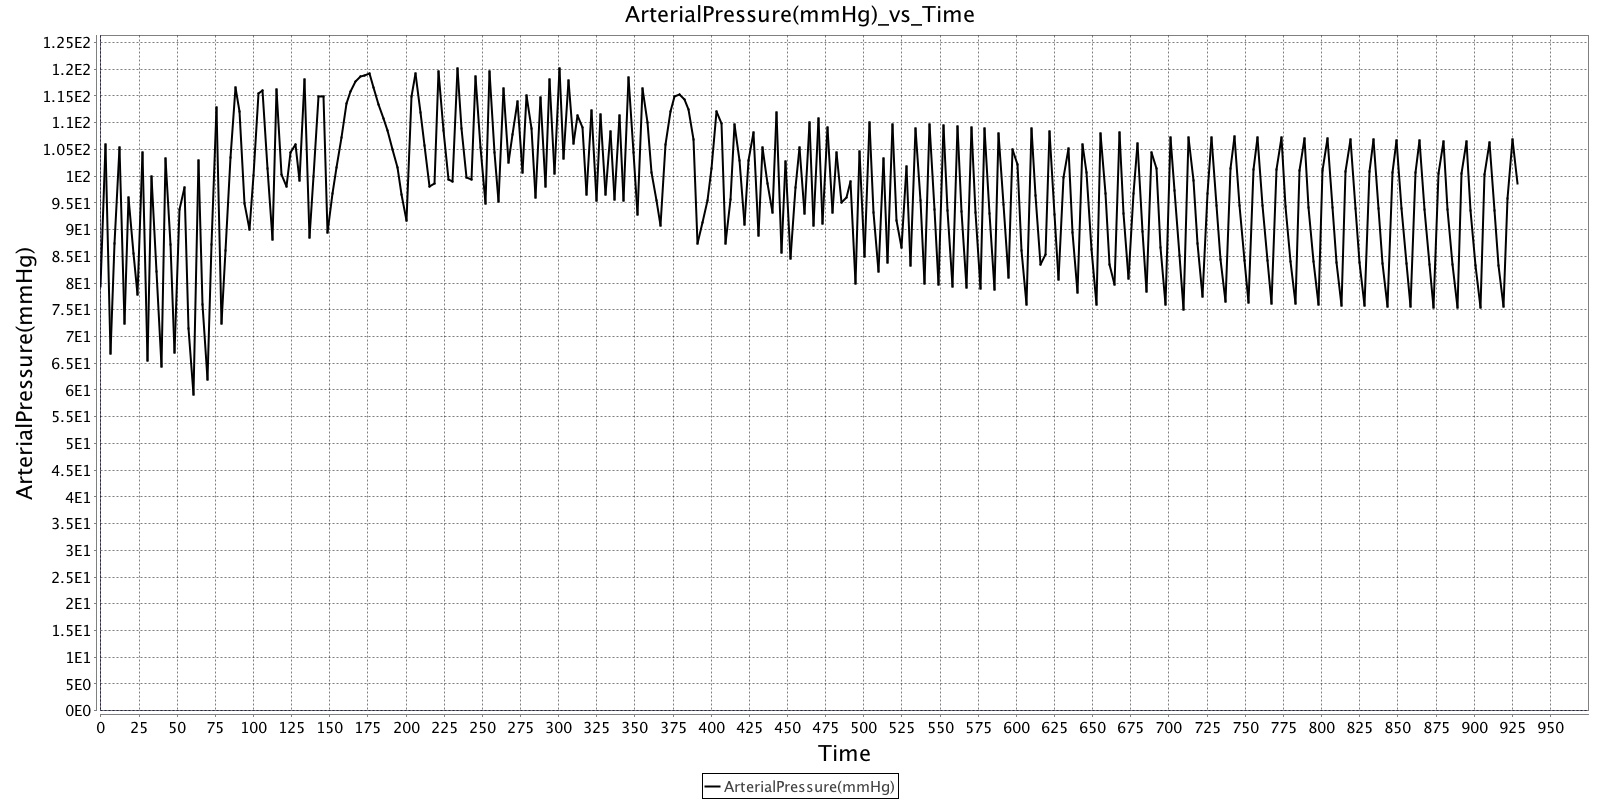
\includegraphics[width=5cm]{Succinylcholine_ArterialPressure_vs_Time.jpg}}
     \caption{Blood Pressure changes}
     \label{fig:given 5 mg Succinylcholine}
     
   \end{minipage}
   \begin {minipage}{0.49\textwidth}
     \frame{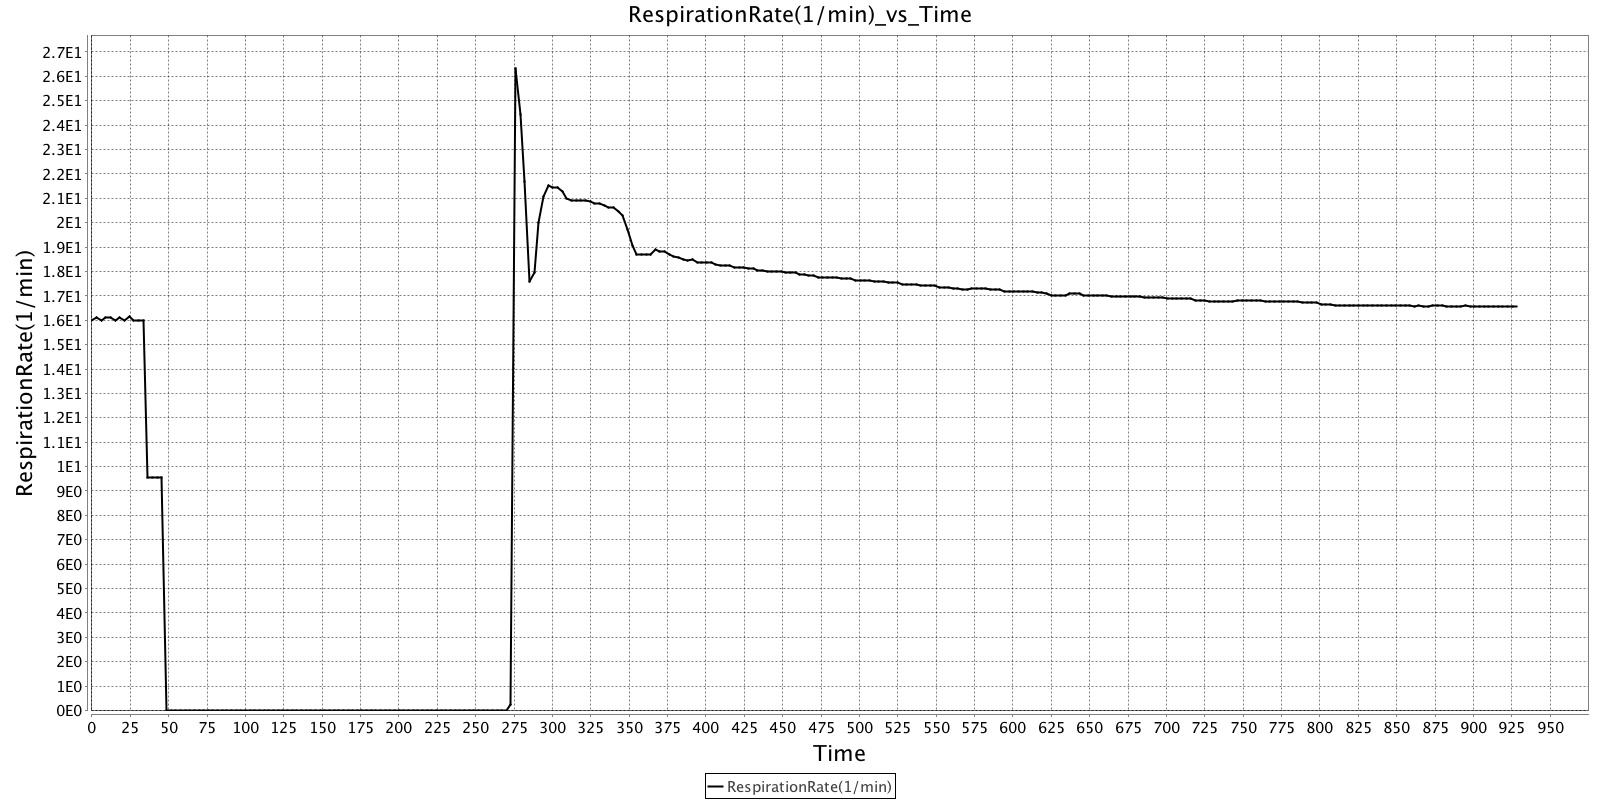
\includegraphics[width=5cm]{Succinylcholine_RespirationRate_vs_Time.jpg}}
     \caption{Respiration Rate changes}
     \label{fig:given 5 mg Succinylcholine}
   \end{minipage}
\end{figure}

In CAE, we set up the Succinycholine's dosage to be 77mg cause Muse only provides options for injection corresponding to the patient weight. We simulated the scenario for 6 minutes. 

\subsubsection{Rocuronium 50 mg Simulation}

Rocuronium is an anaesthesia drug that blocks neuromuscular signals in muscles and therefore used as muscle relaxant. It is widely used for surgery or mechanical ventilation with the nature of rapid onset and intermediate duration. For the experiment, we set up both normal patient and patient with asthma history to see how they react to the drug.(Asthma patient will likely suffer from allergy)

In the experiment, we gave each patient 50 mg Rocuronium and record the response of vital signs as following graphs:

\begin{figure}[!htb]\centering
   \begin{minipage}{0.49\textwidth}
     \frame{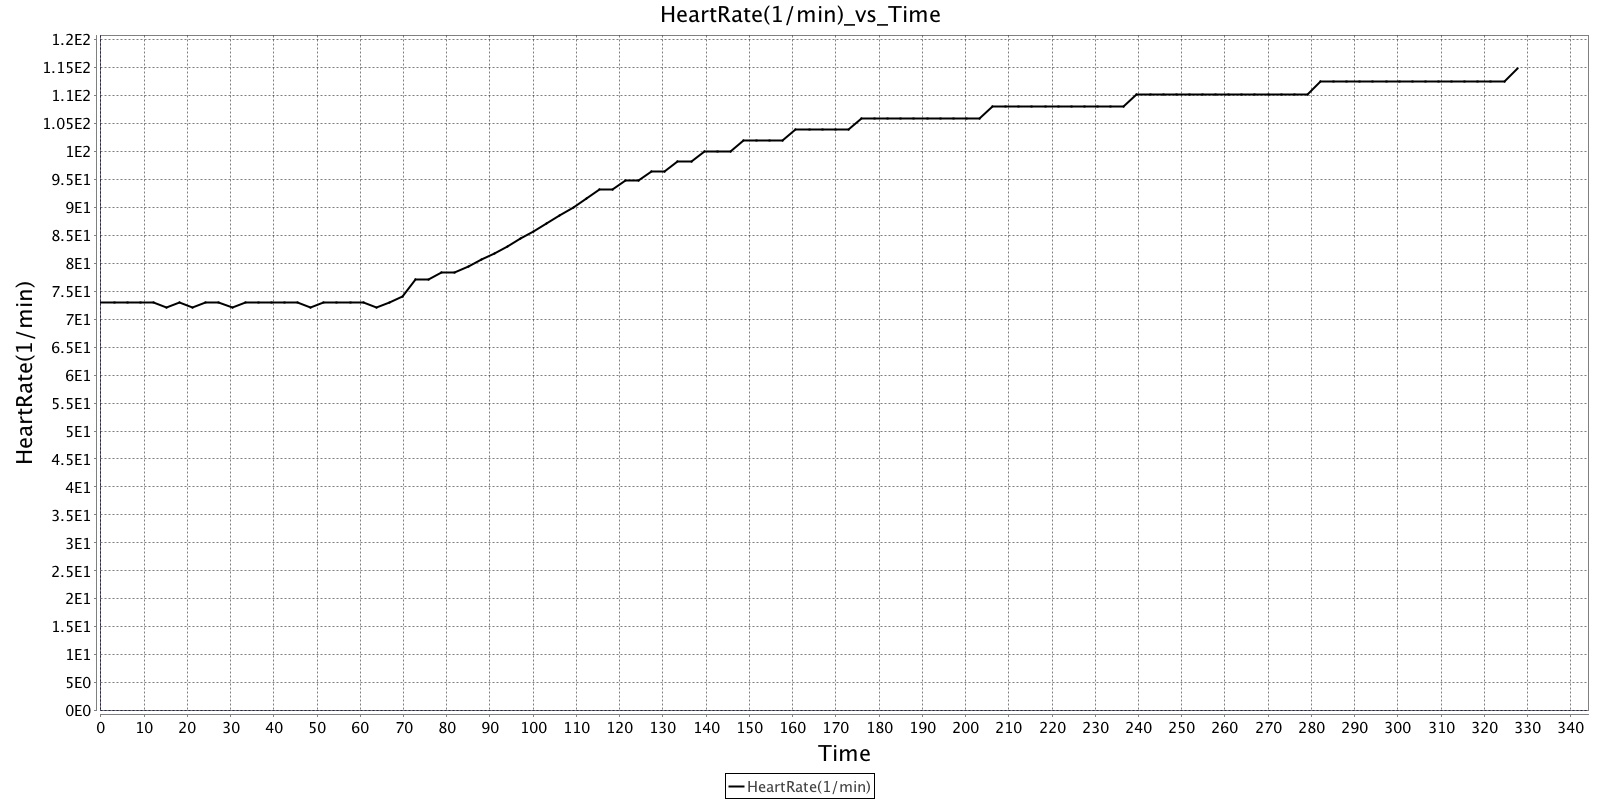
\includegraphics[width=5cm]{Rocuronium_HeartRate_vs_Time.jpg}}
     \caption{Heart Rate changes}
     \label{fig:given 50 mg Rocuronium}
     
   \end{minipage}
   \begin {minipage}{0.49\textwidth}
     \frame{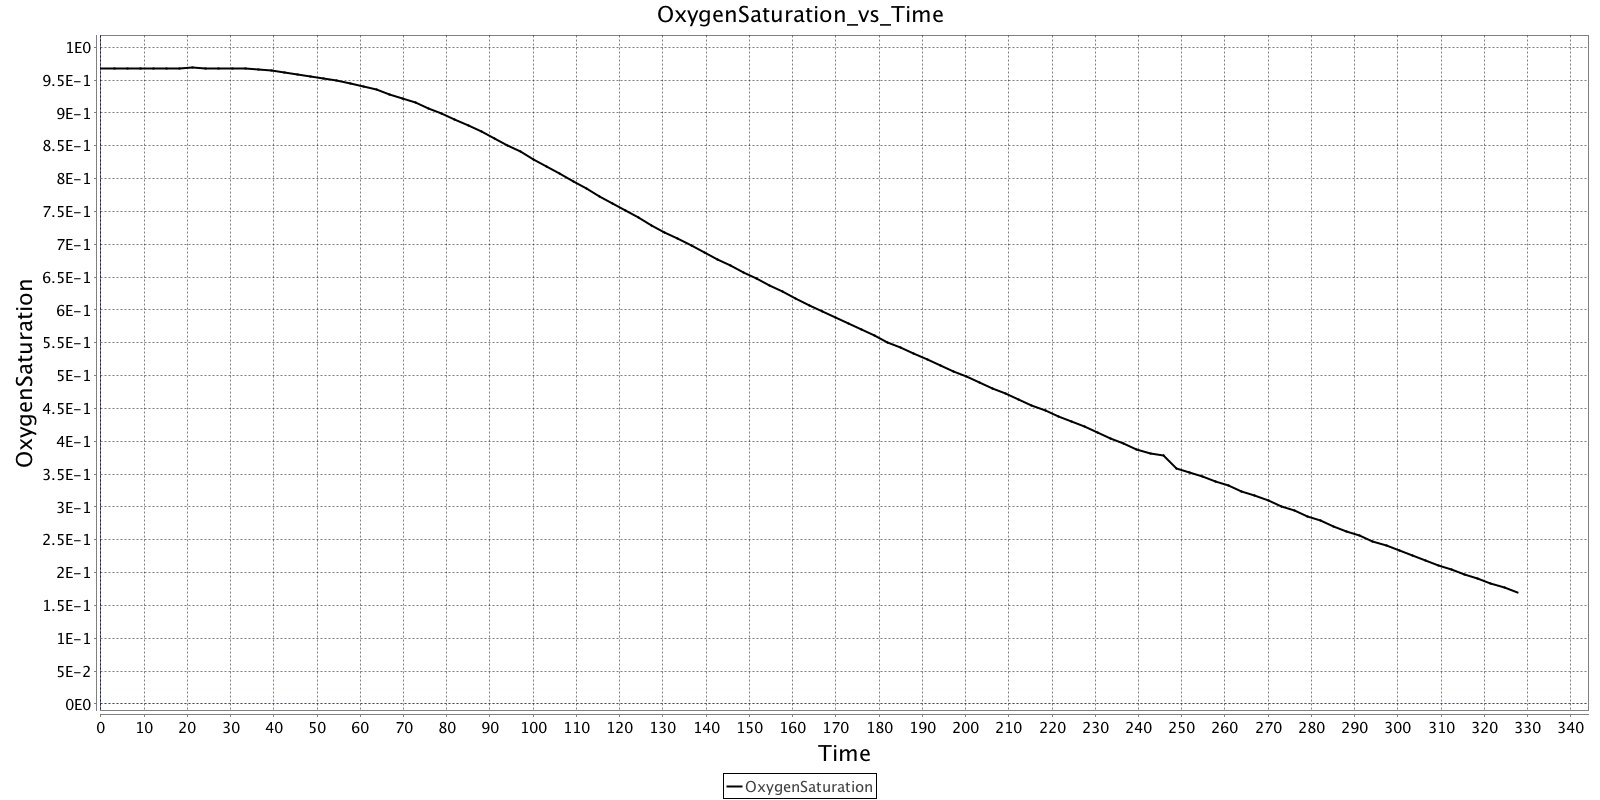
\includegraphics[width=5cm]{Rocuronium_OxygenSaturation_vs_Time.jpg}}
     \caption{Oxygen Saturation changes}
     \label{fig:given 50 mg Rocuronium}
   \end{minipage}
\end{figure}

\begin{figure}[!htb]\centering
   \begin{minipage}{0.49\textwidth}
     \frame{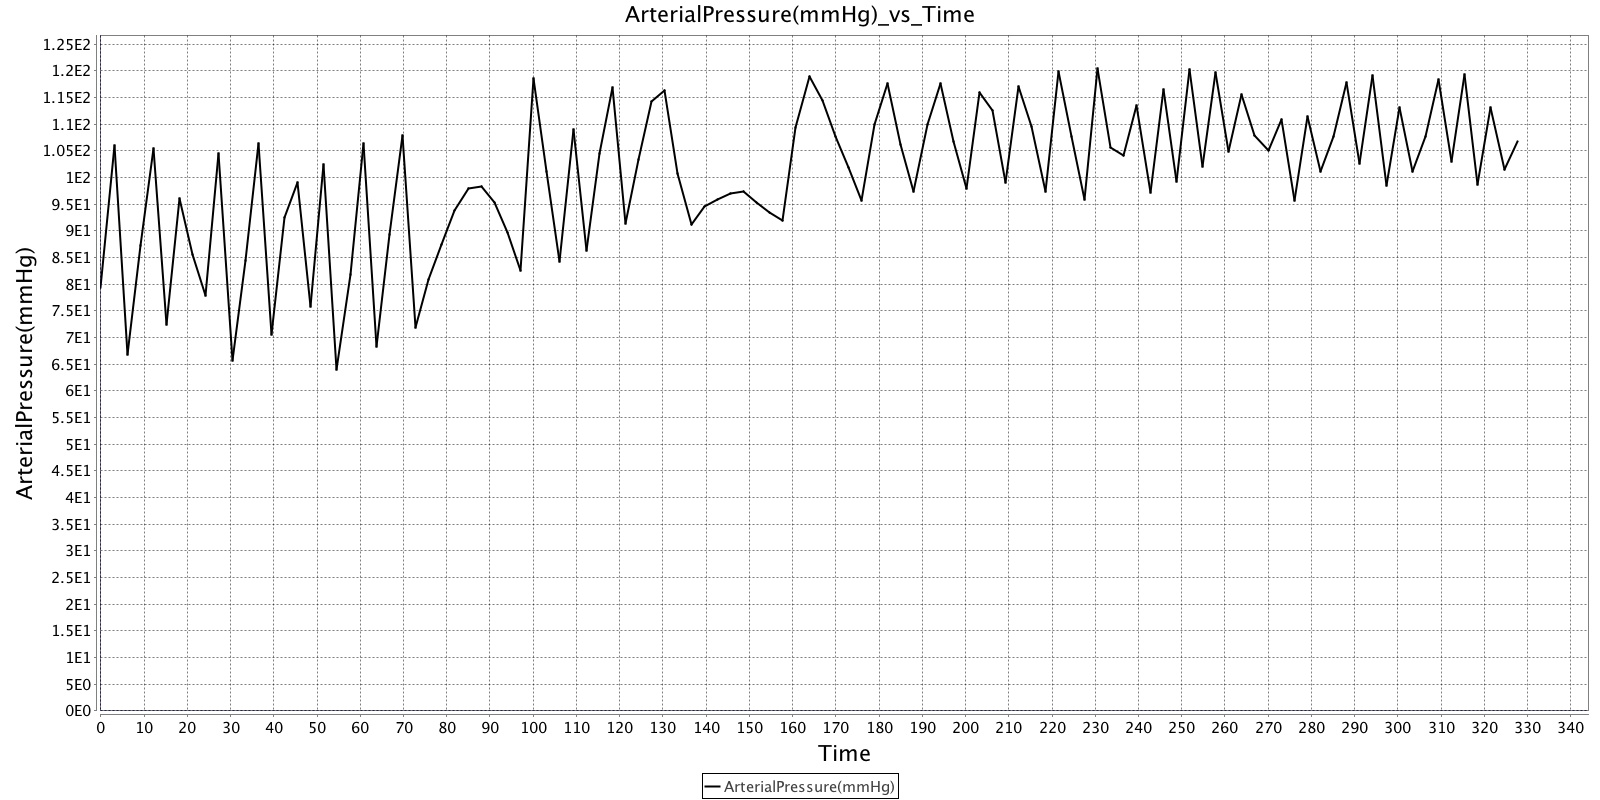
\includegraphics[width=5cm]{Rocuronium_ArterialPressure_vs_Time.jpg}}
     \caption{Blood Pressure changes}
     \label{fig:given 50 mg Rocuronium}
     
   \end{minipage}
   \begin {minipage}{0.49\textwidth}
     \frame{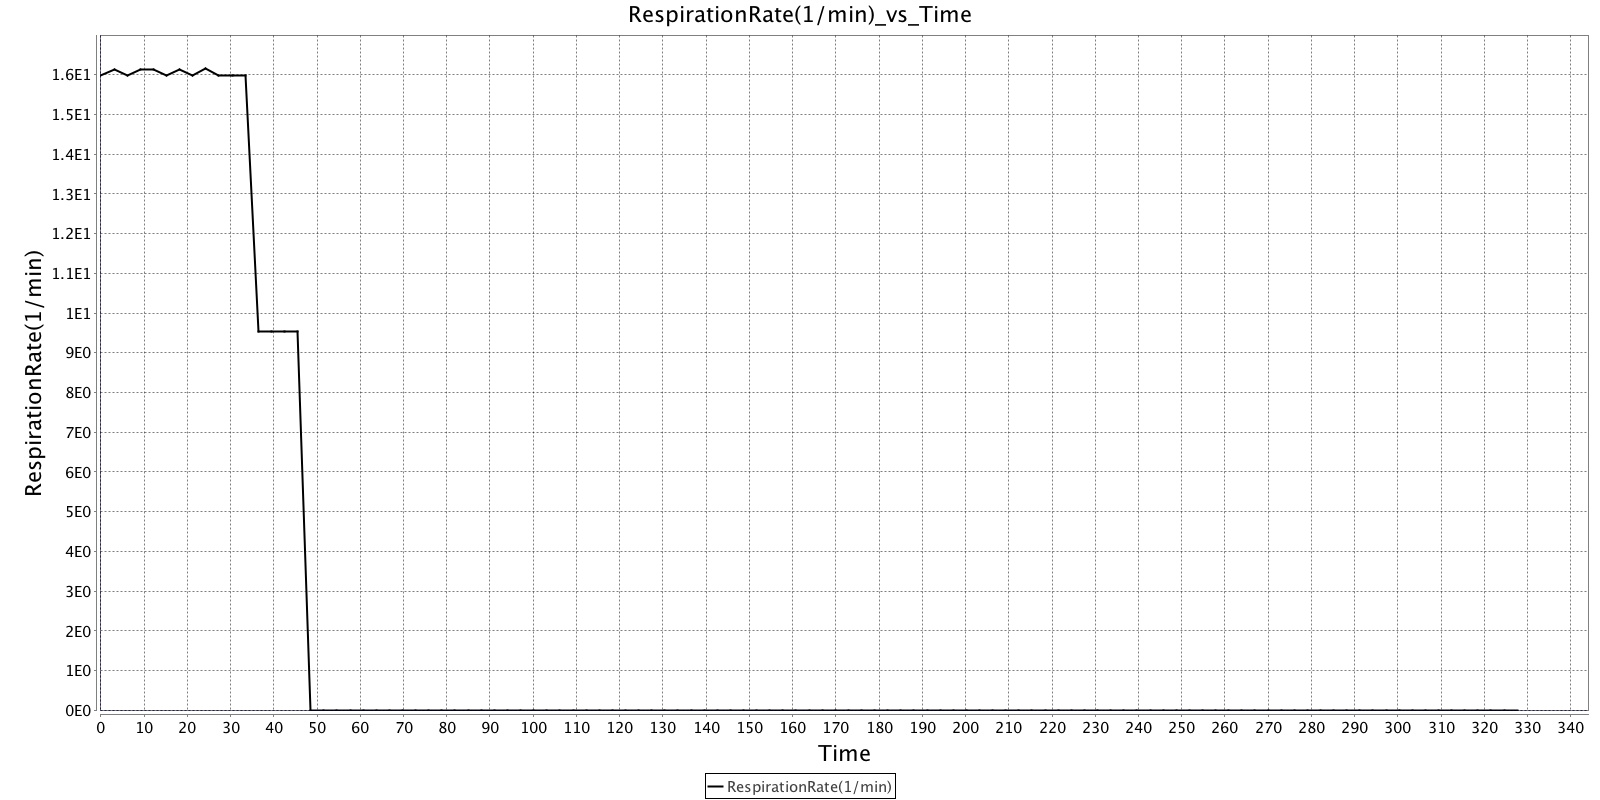
\includegraphics[width=5cm]{Rocuronium_RespirationRate_vs_Time.jpg}}
     \caption{Respiration Rate changes}
     \label{fig:given 50 mg Rocuronium}
   \end{minipage}
\end{figure}
 
\subsubsection{Propofol 200 mg Simulation}

Before and during the surgery, Propofol is widely used as a way of sedation to decrease level of consciousness and lack of memory for events of patients. Its maximum effect usually takes about 2 minutes to take place and it often lasts 5 to 10 minutes.

In our experiment, We set up the dosage to be 200 mg for Biogears and ran it for about 6 mintes. The results are as followed:

\begin{figure}[!htb]\centering
   \begin{minipage}{0.49\textwidth}
     \frame{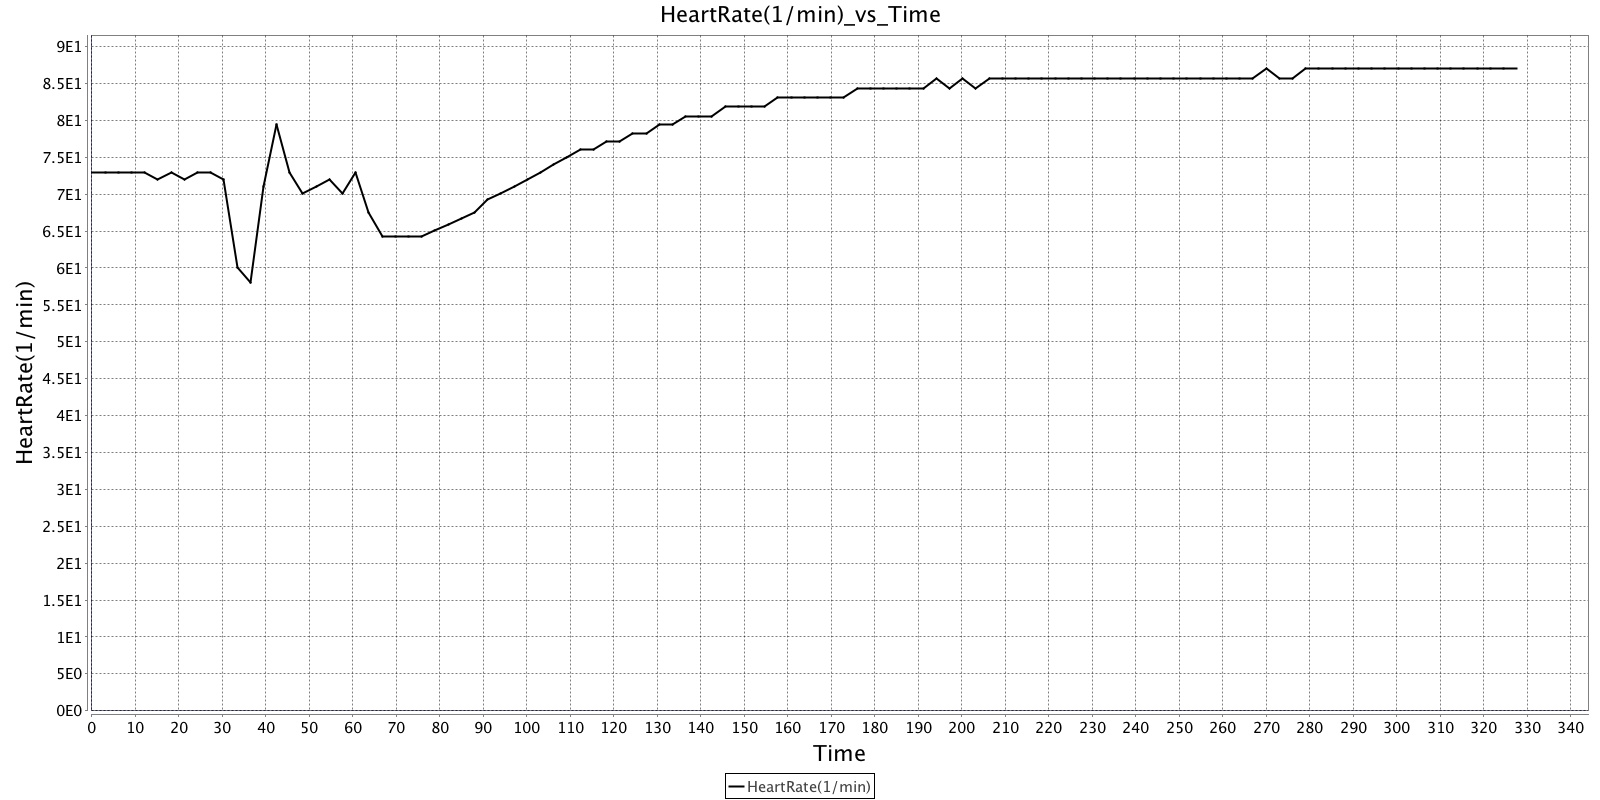
\includegraphics[width=5cm]{Propofol_HeartRate_vs_Time.jpg}}
     \caption{Heart Rate changes}
     \label{fig:given 200 mg Propofol}
     
   \end{minipage}
   \begin {minipage}{0.49\textwidth}
     \frame{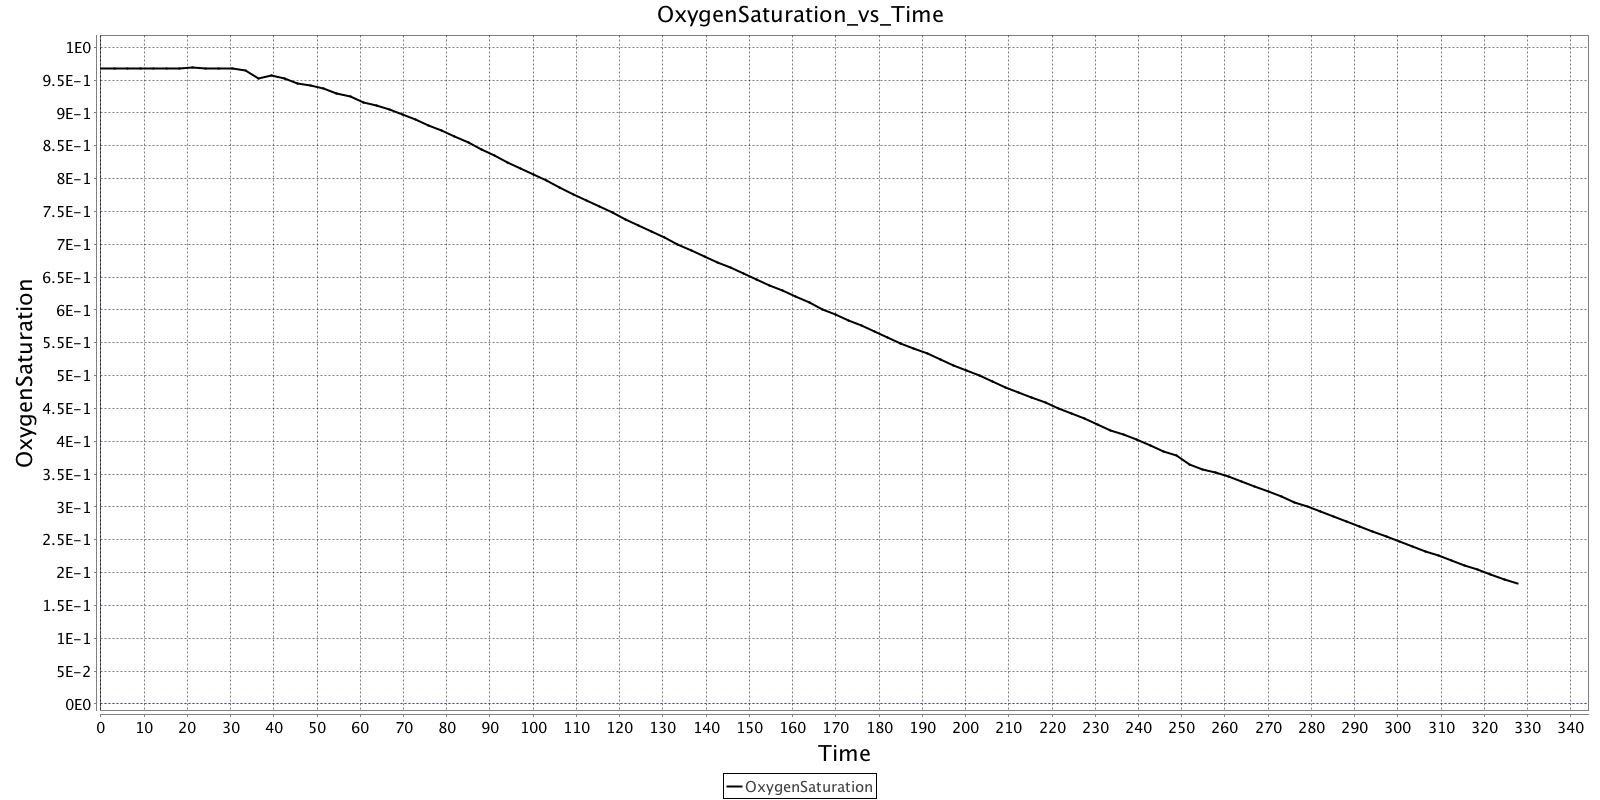
\includegraphics[width=5cm]{Propofol_OxygenSaturation_vs_Time.jpg}}
     \caption{Oxygen Saturation changes}
     \label{fig:given 200 mg Propofol}
   \end{minipage}
\end{figure}

\begin{figure}[!htb]\centering
   \begin{minipage}{0.49\textwidth}
     \frame{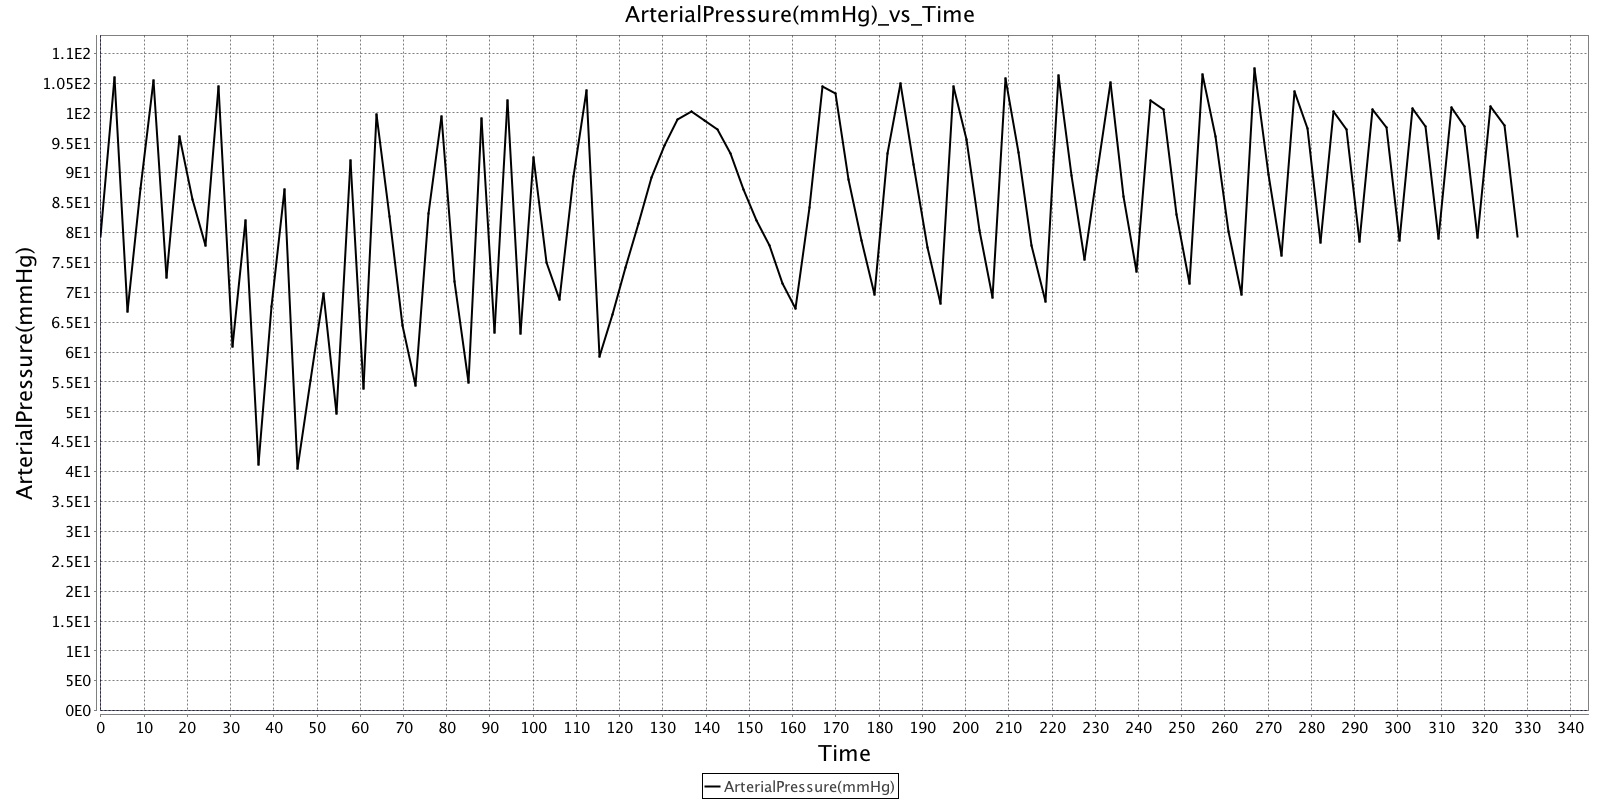
\includegraphics[width=5cm]{Propofol_ArterialPressure_vs_Time.jpg}}
     \caption{Blood Pressure changes}
     \label{fig:given 200 mg Propofol}
     
   \end{minipage}
   \begin {minipage}{0.49\textwidth}
     \frame{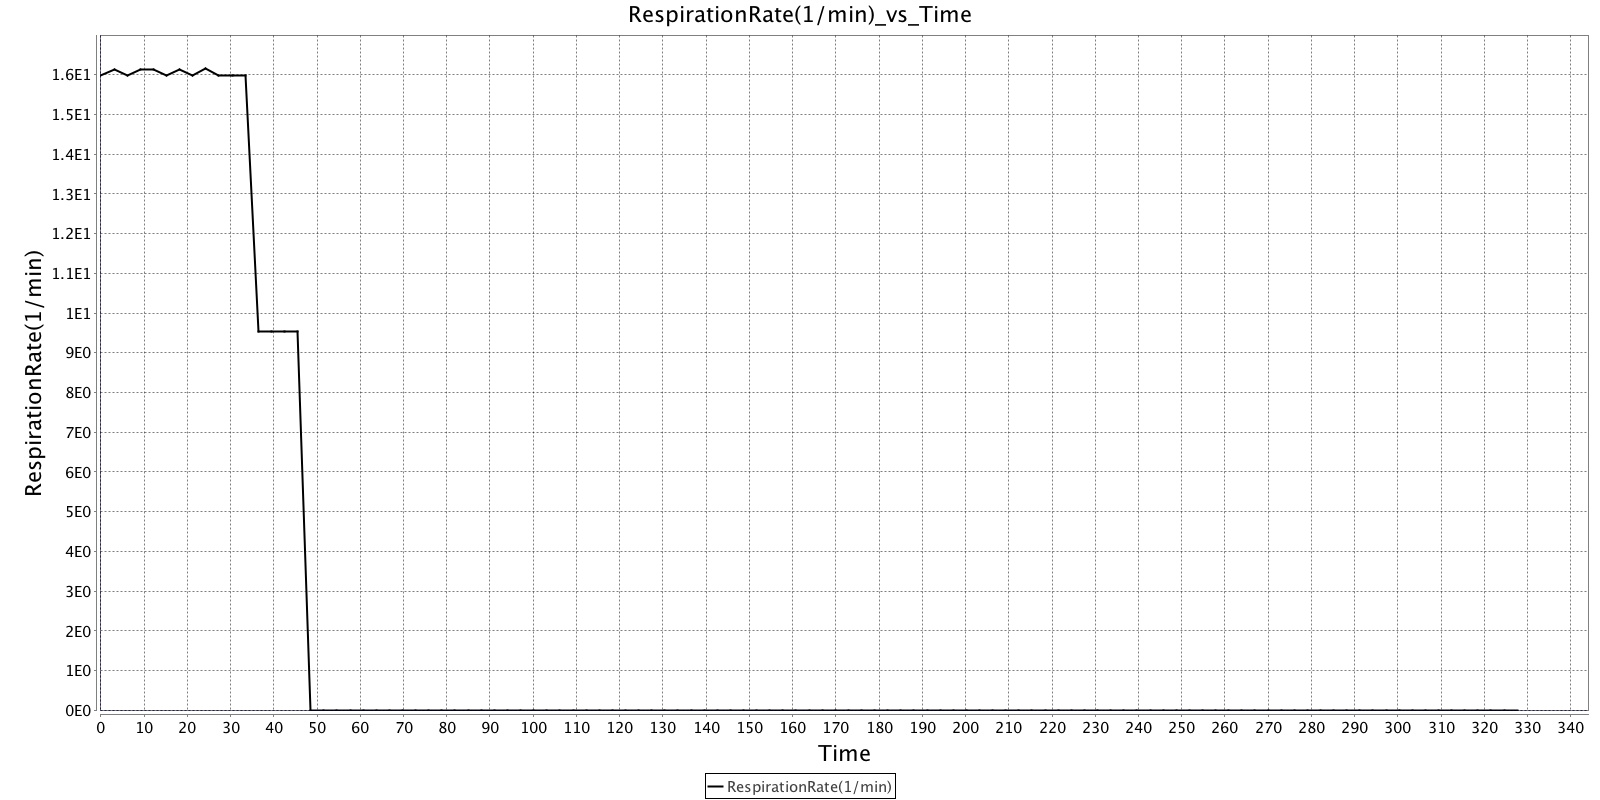
\includegraphics[width=5cm]{Propofol_RespirationRate_vs_Time.jpg}}
     \caption{Respiration Rate changes}
     \label{fig:given 200 mg Propofol}
   \end{minipage}
\end{figure}

\subsubsection{Morphine 40 mg Simulation}

\subsubsection{Fentanyl 500 ug Simulation}

%\subsection{Physical experiments}
%\subsection{Other simulators}

\section{Enumerate limits and future work}
\subsection{Limits of screen based simulation}
\subsection{Future work}

\begin{thebibliography}{1}

  \bibitem{measure_repeatability} Cumin, David, Charlotte Chen, and Alan F. Merry. "Measuring the repeatability of simulated physiology in simulators." Simulation in Healthcare 10.6 (2015): 336-344.

  \bibitem{low_oxygen_sleep}Kearley, R., et al. "The effect of low flow oxygen on sleep-disordered breathing and oxygen desaturation. A study of patients with chronic obstructive lung disease." CHEST Journal 78.5 (1980): 682-685.  

  \bibitem{norman} 

  \bibitem{fo} 

  \end{thebibliography}
\end{document}